 \chapter{Introduction}


Code-breaking games (sometimes also called \emph{deductive games} or \emph{searching games})
  are games of two players in which the first player,
  usually referred to as \emph{the codemaker},
    chooses a secret code from a given set, and the second player,
  usually referred to as \emph{the codebreaker},
    strives to reveal the code through a series
    of experiments that give him partial information about the code.

\begin{wrapfigure}{r}{0.32\textwidth}
  \vspace{-5mm}
  \begin{center}
  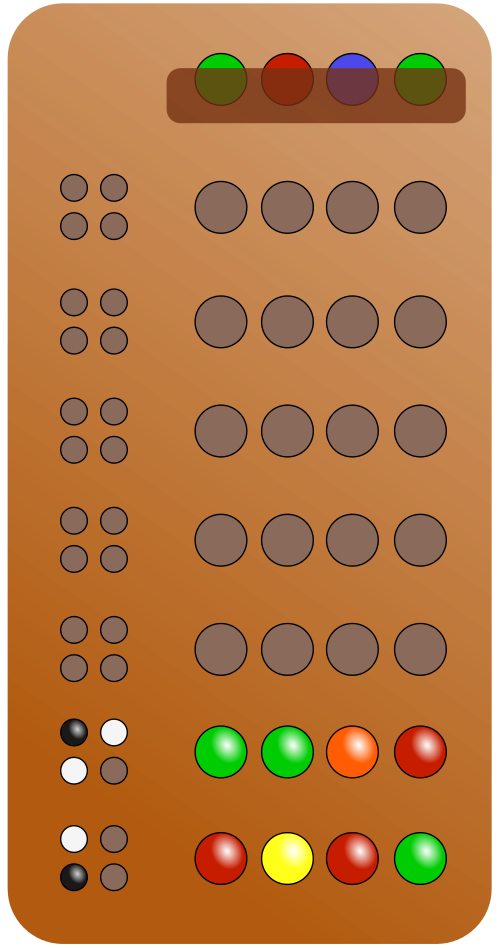
\includegraphics[width=0.25\textwidth]{pictures/mastermind.png}
  \vspace{-5mm}
  \end{center}
  \caption{Mastermind game (illustrative image)\protect\footnotemark.}
  \vspace{-5mm}
\end{wrapfigure}
\footnotetext{Image adopted from \url{http://commons.wikimedia.org/wiki/File:Mastermind\_beispiel.svg}, by Thomas Steiner under GFDL.}

One prominent example of a code-breaking game is famous board game
  \emph{Mastermind}.
In this game, the codemaker creates a puzzle for the codebreaker by choosing a
  combination of four coloured pegs (with colour repetitions allowed).
The codebreaker makes guesses about the colours, which are evaluated by the codemaker with
  black and white markers.
A black marker corresponds to a position where the code and the guess match.
A white marker means that some colour is present both in the code
  and in the guess but at different positions.

Another example of a code-breaking game is the \emph{counterfeit coin problem},
  the problem of identifying an odd-weight coin among
  a collection of genuine coins using only a balance scale.
The codemaker is not a real player here; the balance scale takes his function
  and evaluates the weighings performed by the codebreaker.
Numerous other examples can be found among various board games and logic puzzles;
 we present some of them in the next chapter.

Code-breaking games offer many interesting research problems.

\begin{itemize}
\item \emph{How should the codebreaker play in order to minimize the number of experiments
   needed to undoubtedly determine the code?}
\item \emph{Is there a strategy that would guarantee
   revealing the code in at most $k$ steps?}
\item \emph{What strategy is optimal with respect
   to the average-case number of experiments,
   given that the code is selected
   from the given set with uniform distribution?}
\end{itemize}

Synthesis of an optimal strategy is a computationally intensive task.
In some games, the optimal strategy might have a simple
  structure and can be described easily, such as in
  the counterfeit coin problem (see section \autoref{s:coins} for details).
In general, however, the strategy may have complicated structure and
  the there may be no other way to discover an optimal strategy
  than to consider all possible experiments
  in a given state and analyse the subproblems.

Therefore, one may prefer a suboptimal strategy or heuristic
  for experiment selection, which is easier to compute.
This brings about another kind of questions.
\emph{Given a strategy,
  how can we compute the worst-case and the average-case number
  of experiments the strategy needs to reveal the code?}

Some particular code-breaking games,
  such as Mastermind and the counterfeit coin problem,
  have been intensively studied in the last decades
  and most of these questions are at least partially answered.
A detailed summary of the existing results is presented in \autoref{ch:games}.
Nevertheless, little has been written about code-breaking games in general.
Some authors have suggested general methods (and applied them in one particular game,
  e.g. \cite{cbg-stgopt, cbg-gen}),
  some have vaguely stated that their approach can be applied
  to other games of the same kind but,
  to the best of our knowledge, no one has tried to
  create a general framework and provide
   results for code-breaking games in general.

This work proposes to bridge the gap and provides
  a general framework for code-breaking games
  based on propositional logic.
The secret code is encoded as a valuation of
  a set of propositional variables
  and the codebreaker's goal is to discover the valuation
  through a series of experiments.
Each experiment can result in several outcomes,
  which are given in the form of a propositional formula.

We address the following challenges in the suggested framework.
\begin{itemize}
\item Formally define code-breaking games and strategies.
\item Propose general strategies or heuristics for experiment selection.
\item Suggest efficient methods for state-space reduction based on symmetry detection.
\item Propose algorithms for strategy evaluation and optimal strategy synthesis.
\item Design a computer language for game specification.
\item Develop a computer program that parses a game description from the
  designed language and implements suggested algorithms.
\end{itemize}

Suggested methods for code-breaking game analysis depend
  on algorithms for some related problems.
To analyse propositional formulas emerging during the course of the game,
  we need to decide satisfiability or count the number of models of
  a formula, which can be done using a modern SAT solver.
Further, our symmetry detection approach is based on the reduction
  of experiment equivalence to graph isomorphism.
For this purpose, we need a tool that computes the canonical labelling of a graph.

% exploit symmetries in the game
% Algorithms for symmetry detection in Mastermind
%   based on graph isomorphism have been suggested in \cite{cbg-nauty}.
% \item verifying that a game specification is correct
%   and sensible (overview mode),

We created a computer program for code-breaking game analysis and named it COBRA,
  the code-breaking game analyser.
Using this tool, we can reproduce some of the existing results
  for Mastermind, analyse new code-breaking games and and easily evaluate new heuristics
  for experiment selection.

The thesis is structured as follows.
\autoref{ch:games} introduces several examples of code-breaking games and
  discusses existing results, variants of the games and related research.
The general code-breaking game model is described in \autoref{ch:model}.
\autoref{ch:expeq} is dedicated to the method for symmetry detection and other algorithms.
Our computer program, COBRA, with descriptions of its usage and
  abilities is introduced in \autoref{ch:cobra}.
Experimental results with comparisons of analysed strategies
  are presented in \autoref{ch:exp}.
Finally, \autoref{ch:conclusions} concludes the work with suggestions for future work
  and possible extensions of the tool.






